%%%%%%%%%%%%%%%%%%%%%%%%%%%%%%%%%%%%%%%%%%%%%
\section{Results for fixed angular momentum}
\label{Sec:FixedL}
%%%%%%%%%%%%%%%%%%%%%%%%%%%%%%%%%%%%%%%%%%%%%

In this section we apply the methods of section~\ref{Sec:Numerics} to the reduced model in which all the gas particles have the same magnitude $L_0$ of the angular momentum. We start with the two families of self-consistent steady states whose perturbations are analyzed, and with the dependency of their frequency bands on the mass of the gas. Next, we compute the gain $\lambda(\omega)$ of the self-consistent loop, verify its behavior at the edge of the band, and determine the threshold mass above which an oscillating mode exists. Then, we analyze the response of the gas to the perturbation~(\ref{Eq:InitialData}), first below the threshold, where it decays, and afterwards above it, where it settles down to an oscillation which is not damped, and in each case we compare the results which are obtained from the PIC code, from the linearized equations and from the gain. Finally, we show that the dependency of the response on the amplitude of the perturbation which was found in section~\ref{SubSec:ValResponse} is due to the trapping of the gas particles near the edge of the steady state by the oscillating mode, and we estimate the amplitude above which this occurs.


\subsection{Steady states}
\label{SubSec:FixedLStates}

We consider the two families of self-consistent steady states introduced in section~\ref{SubSec:SteadyStatesNum}. The first one consists of the lowered Maxwellians~(\ref{Eq:LoweredMaxwellian}) with $W_0 = 3$ in the isochrone potential, for $L_0 = 2$. Unless otherwise stated we choose $g = 2$ and $J_{max} = 0.138$, and we vary the mass of the gas in the range $0.003\leq M_{gas}/M\leq 0.5$. In the limit $M_{gas}/M\to 0$, Eq.~(\ref{Eq:OmegaIsochrone}) with $c(L_0) = 1 + \sqrt{2}$ yields the frequency band $[\Omega_{min},\Omega_{max}] = [0.0602,0.0711]$, whose width is only $17$ percent of its mean value, and the gas occupies the shell $4.3 < r < 8.5$. In order to analyze the dependency of the results on the width of the band and on the behavior of the DF at the edge of its support, we also consider $J_{max} = 0.083$ and $J_{max} = 0.276$, as well as the exponents $g = 0.75$, $1$, $1.5$ and $3$.

The second family consists of the polytropes~(\ref{Eq:Polytrope}) in the Kepler potential with $k = 0.75$, $1$, $1.25$, $1.5$, $2$ and $3$, for $L_0 = 2$, $J_{max} = 0.7$ and $0.01\leq M_{gas}/M\leq 1$. These are the steady states for which the dichotomy of Ref.~\cite{mHgRmScS25} has been established. Recall that in the Kepler case the value of $L_0$ can be fixed by means of the rescaling~(\ref{Eq:Rescaling}), such that this family is characterized by $k$, $J_{max}/L_0$ and $M_{gas}/M$. In the limit $M_{gas}/M\to 0$ the frequency band is $[0.0508,0.125]$ and the gas occupies the shell $2.4 < r < 12.2$. Hence, in contrast to the first family, the band is wide: $\Omega_{max}/\Omega_{min} = 2.46$.

\begin{table}[htp]
\begin{center}
\begin{tabular}{ll|cc|cc|cc}
\hline\hline
 & $M_{gas}/M$ & $r_{in}$ & $r_{out}$ & $\Omega_{min}$ & $\Omega_{max}$ & $\lambda(0)$ & $\lambda_{edge}$ \\
\hline
lowered Maxwellian, $g = 2$ & $0.0065$ & $4.31$ & $8.50$ & $0.06097$ & $0.07230$ & $0.018$ & $0.100$ \\
 & $0.042$ & $4.25$ & $8.29$ & $0.06548$ & $0.07915$ & $0.105$ & $0.555$ \\
 & $0.058$ & $4.23$ & $8.20$ & $0.06756$ & $0.08230$ & $0.140$ & $0.720$ \\
 & $0.075$ & $4.20$ & $8.11$ & $0.06979$ & $0.08570$ & $0.174$ & $0.874$ \\
 & $0.097$ & $4.17$ & $7.99$ & $0.07271$ & $0.09017$ & $0.215$ & $1.047$ \\
 & $0.17$ & $4.06$ & $7.63$ & $0.08275$ & $0.10552$ & $0.326$ & $1.468$ \\
 & $0.5$ & $3.60$ & $6.40$ & $0.13419$ & $0.18434$ & $0.586$ & $2.210$ \\
\hline
polytrope, $k = 0.75$ & $0.01$ & $2.39$ & $12.10$ & $0.05159$ & $0.12618$ & $0.008$ & $\infty$ \\
\phantom{polytrope,} $k = 1$ & $0.01$ & $2.39$ & $12.10$ & $0.05161$ & $0.12626$ & $0.008$ & $\infty$ \\
\phantom{polytrope,} $k = 1.5$ & $0.01$ & $2.39$ & $12.10$ & $0.05163$ & $0.12640$ & $0.009$ & $0.018$ \\
\phantom{polytrope,} $k = 2$ & $0.01$ & $2.39$ & $12.09$ & $0.05165$ & $0.12652$ & $0.010$ & $0.016$ \\
\hline
polytrope, $k = 0.75$ & $1$ & $1.83$ & $7.57$ & $0.15159$ & $0.28367$ & $0.387$ & $\infty$ \\
\phantom{polytrope,} $k = 1$ & $1$ & $1.81$ & $7.50$ & $0.15399$ & $0.29366$ & $0.402$ & $\infty$ \\
\phantom{polytrope,} $k = 1.25$ & $1$ & $1.80$ & $7.45$ & $0.15601$ & $0.30303$ & $0.415$ & $1.583$ \\
\phantom{polytrope,} $k = 1.5$ & $1$ & $1.79$ & $7.40$ & $0.15774$ & $0.31186$ & $0.428$ & $1.051$ \\
\phantom{polytrope,} $k = 2$ & $1$ & $1.78$ & $7.32$ & $0.16053$ & $0.32814$ & $0.452$ & $0.820$ \\
\phantom{polytrope,} $k = 3$ & $1$ & $1.75$ & $7.21$ & $0.16434$ & $0.35648$ & $0.492$ & $0.738$ \\
\hline\hline
\end{tabular}
\end{center}
\caption{Properties of the self-consistent steady states of the reduced model whose perturbations are analyzed in this section: the lowered Maxwellians~(\ref{Eq:LoweredMaxwellian}) with $W_0 = 3$ and $J_{max} = 0.138$ in the isochrone potential, and the polytropes~(\ref{Eq:Polytrope}) with $J_{max} = 0.7$ in the Kepler potential, in both cases with $L_0 = 2$. Shown are the inner and outer radii of the shell which is occupied by the gas, the frequency band, and the gain of the self-consistent loop at zero frequency and at the edge of the band.}
\label{Tab:SteadyStates}
\end{table}

The properties of the steady states to which the simulations of this section refer are summarized in Table~\ref{Tab:SteadyStates}. As the mass of the gas increases, the potential well becomes deeper, the gas contracts, and the frequencies of all the orbits grow. For the lowered Maxwellians, $\Omega_{min}$ increases from $0.0605$ for $M_{gas}/M = 0.003$ to $0.134$ for $M_{gas}/M = 0.5$, and the ratio $\Omega_{max}/\Omega_{min}$ from $1.18$ to $1.37$. For the polytropes with $M_{gas}/M = 1$, $\Omega_{min}$ is about three times larger than for vanishing mass, and $\Omega_{max}/\Omega_{min}$ lies between $1.87$ and $2.17$.

For all these steady states the DF is a decreasing function of the energy, such that the considerations of section~\ref{SubSec:Gain} apply. The gain at zero frequency increases with the mass of the gas (see Table~\ref{Tab:SteadyStates}); its largest value, $\lambda(0) = 0.586$, is attained for the lowered Maxwellian with $M_{gas}/M = 0.5$. Therefore, all the steady states considered here are linearly stable with respect to spherically symmetric perturbations. Furthermore, the second largest eigenvalue of the operator $S(\omega)$, which also increases with $\omega$, is smaller than $0.26$ in all the cases. Its largest value at the edge of the band, $0.258$, is again attained for the lowered Maxwellian with $M_{gas}/M = 0.5$. For the steady states with $k\leq 1$, for which the largest eigenvalue diverges at the edge, we have evaluated the second one up to the distance $10^{-12}(\Omega_{max} - \Omega_{min})$ from the edge, where it is equal to $0.230$ and $0.246$ for the polytropes with $M_{gas}/M = 1$ and $k = 0.75$ and $k = 1$, respectively. Hence, there is at most one oscillating mode with frequency below the band.

In the remainder of this section the response of the gas to the perturbation~(\ref{Eq:InitialData}) is described by the function $\chi_1(t)$ defined in Eq.~(\ref{Eq:Response}), which is computed with the weight function~(\ref{Eq:BDef}) with $J_1 = \sigma_1 = 0.05$ for the lowered Maxwellians and with $J_1 = 0.35$ and $\sigma_1 = 0.2$ for the polytropes. With these choices $|\chi_1(0)| = 0.138$ in the first case and $0.17\leq |\chi_1(0)|\leq 0.22$ in the second one. The PIC simulations use $N_J\times N_Q = 400\times 25$ and $\Delta r = 0.1$, with $\Delta t = 0.05$ for the lowered Maxwellians and $\Delta t = 0.1$ for the polytropes, except for the polytrope with $k = 1.25$ and $M_{gas}/M = 1$, for which we use the simulations with $N_J\times N_Q = 1280\times 80$ and $\Delta t = 0.05$ of section~\ref{SubSec:ValResponse}.


\subsection{Gain of the self-consistent loop and threshold mass}
\label{SubSec:FixedLGain}

We have computed the gain $\lambda(\omega)$ with the method of section~\ref{SubSec:GainNum} for all the steady states of the previous subsection. In the following we measure the distance of a frequency $\omega < \Omega_{min}$ from the edge of the band in units of the width of the band,
\begin{equation}
\delta := \frac{\Omega_{min} - \omega}{\Omega_{max} - \Omega_{min}},
\label{Eq:deltaDef}
\end{equation}
and we denote by $\delta_d$ the value of this quantity for the frequency $\omega_d$ of an oscillating mode.

\begin{figure}[htp]
\centerline{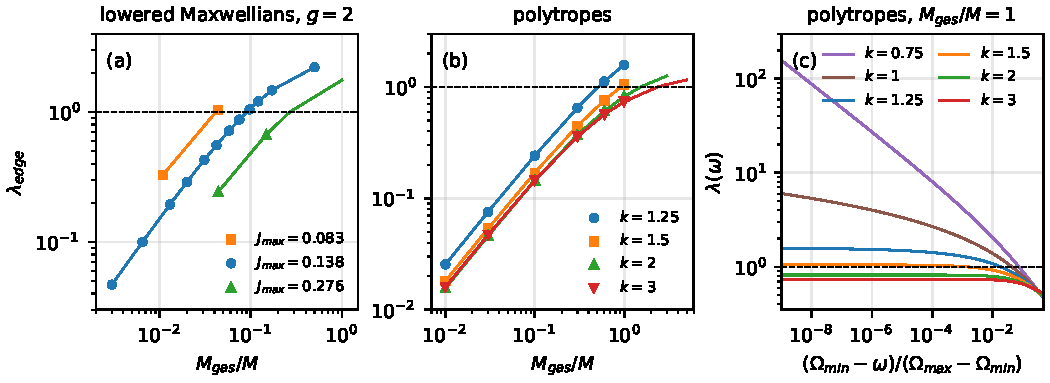
\includegraphics[width=\textwidth]{figuras/resultados_ganancia.pdf}}
\caption{Gain of the self-consistent loop. (a) The value $\lambda_{edge}$ at the edge of the frequency band as a function of the mass of the gas, for the lowered Maxwellians with $g = 2$ in the isochrone potential and three values of $J_{max}$. (b) The same for the polytropes with $k > 1$ in the Kepler potential. The symbols refer to the steady states of section~\ref{SubSec:FixedLStates}, and the lines include those which were computed in order to determine the threshold mass. (c) The gain as a function of the distance~(\ref{Eq:deltaDef}) from the edge of the band, for the polytropes with $M_{gas}/M = 1$. An oscillating mode exists if and only if the curve crosses the dashed line $\lambda = 1$.}
\label{Fig:Gain}
\end{figure}

We first verify the behavior of the gain at the edge of the band which was derived in section~\ref{SubSec:Edge}. Figure~\ref{Fig:Gain}(c) shows $\lambda$ as a function of $\delta$ for the polytropes with $M_{gas}/M = 1$. For $k > 1$ the gain converges to a finite value when $\delta\to 0$, whereas for $k\leq 1$ it grows without bound. In the interval $10^{-8}\leq \delta\leq 10^{-5}$ the logarithmic derivative $d\log\lambda/d\log\delta$ lies between $-0.261$ and $-0.252$ for $k = 0.75$, and $d\lambda/d\log(1/\delta)$ lies between $0.288$ and $0.290$ for $k = 1$, which corresponds to the laws $\delta^{k-1}$ and $|\log\delta|$, respectively. For $k > 1$, the local exponent $d\log(\lambda_{edge} - \lambda)/d\log\delta$ in the same interval lies between $0.249$ and $0.250$ for $k = 1.25$, between $0.49$ and $0.50$ for $k = 1.5$, between $0.92$ and $0.95$ for $k = 2$, and it is equal to $1.000$ for $k = 3$, in agreement with the exponent $\min\{ k-1,1 \}$ and with the logarithmic correction for $k = 2$.

Next, we consider the dependency of $\lambda_{edge}$ on the mass of the gas, which is shown in Figs.~\ref{Fig:Gain}(a) and (b). For small masses $\lambda_{edge}$ is proportional to $M_{gas}/M$, as explained in section~\ref{SubSec:Edge}: the ratio between both quantities is $15.6$ for the lowered Maxwellians with $g = 2$ and $J_{max} = 0.138$, and $2.55$, $1.81$, $1.57$ and $1.60$ for the polytropes with $k = 1.25$, $1.5$, $2$ and $3$, respectively. For larger masses the growth is slower, since the frequencies of the orbits increase with the mass of the gas; for the lowered Maxwellian with $M_{gas}/M = 0.5$ the ratio has decreased to $4.4$. Nevertheless, in all the cases $\lambda_{edge}$ increases monotonically with the mass and reaches the value one at a threshold mass. We have determined it by solving the equation $\lambda_{edge} = 1$ with a bracketing root finder, computing a self-consistent steady state for each trial value of the mass. The results are given in Table~\ref{Tab:Threshold}.

\begin{table}[htp]
\begin{center}
\begin{tabular}{ll|c|cc}
\hline\hline
 & & threshold $M_{gas}/M$ & $\Omega_{min}$ & $\Omega_{max}$ \\
\hline
lowered Maxwellian, $g = 2$ & $J_{max} = 0.083$ & $0.0416$ & $0.0705$ & $0.0807$ \\
 & $J_{max} = 0.138$ & $0.0906$ & $0.0719$ & $0.0889$ \\
 & $J_{max} = 0.276$ & $0.268$ & $0.0794$ & $0.1150$ \\
\hline
polytrope & $k = 1.25$ & $0.514$ & $0.0989$ & $0.2057$ \\
 & $k = 1.5$ & $0.920$ & $0.1473$ & $0.2935$ \\
 & $k = 2$ & $1.53$ & $0.2390$ & $0.4737$ \\
 & $k = 3$ & $2.38$ & $0.4095$ & $0.8526$ \\
\hline\hline
\end{tabular}
\end{center}
\caption{Threshold mass, defined by the condition $\lambda_{edge} = 1$, above which an oscillating mode with frequency below the band exists, and frequency band of the steady state at the threshold. For the lowered Maxwellians with $g\leq 1$ and for the polytropes with $k\leq 1$, $\lambda_{edge}$ is infinite and a mode exists for any mass.}
\label{Tab:Threshold}
\end{table}

For the lowered Maxwellians with $g = 2$ and $J_{max} = 0.138$ the threshold is $M_{gas}/M = 0.0906$. It decreases to $0.0416$ when the support of the DF is narrowed to $J_{max} = 0.083$, and it increases to $0.268$ for $J_{max} = 0.276$. For the polytropes the threshold is much larger: it is $0.514$ for $k = 1.25$ and $0.920$ for $k = 1.5$, and for $k = 2$ and $k = 3$ an oscillating mode only exists when the gas is more massive than the central object, namely for $M_{gas}/M > 1.53$ and $M_{gas}/M > 2.38$, respectively. The difference between the two families can be attributed to the width of the frequency band, which is much larger for the polytropes: the narrower the band, the smaller the perturbation of the potential which is required in order to keep the orbits in phase. For the same reason, within the first family the threshold grows with $J_{max}$.

At a fixed mass, the existence of the mode is controlled by the behavior of the DF at the edge. For the lowered Maxwellians with $J_{max} = 0.138$ and masses in the range $0.074\leq M_{gas}/M\leq 0.078$ we obtain $\lambda_{edge} = 0.772$, $0.874$ and $1.051$ for $g = 3$, $2$ and $1.5$, respectively, and for $g\leq 1$ it is infinite; likewise, for the polytropes with $M_{gas}/M = 1$, $\lambda_{edge}$ increases from $0.738$ for $k = 3$ to $1.583$ for $k = 1.25$ (see Table~\ref{Tab:SteadyStates}). Hence, the less regular the DF is at the edge of its support, the larger is the gain.

When $\lambda_{edge} > 1$, the frequency of the mode follows from Eq.~(\ref{Eq:ModeFrequency}). Slightly above the threshold it lies just below the band: $\delta_d = 0.012$ for the lowered Maxwellian with $M_{gas}/M = 0.097$, and $\delta_d = 1.5\times 10^{-3}$ for the polytrope with $k = 1.5$ and $M_{gas}/M = 1$. As the mass increases, the mode separates from the band; for the lowered Maxwellians we find $\delta_d = 0.072$, $0.19$ and $0.59$ for $M_{gas}/M = 0.121$, $0.17$ and $0.5$, respectively. The frequencies $\omega_d$ are listed in Table~\ref{Tab:Modes} below.

For $k\leq 1$ an oscillating mode exists for any mass of the gas. However, when the mass is small its frequency lies extremely close to $\Omega_{min}$, as anticipated in Eq.~(\ref{Eq:Binding}). For the polytropes with $k = 0.75$ we find $\delta_d = 2.0\times 10^{-8}$, $1.5\times 10^{-6}$, $1.3\times 10^{-4}$, $4.4\times 10^{-3}$, $0.027$ and $0.075$ for $M_{gas}/M = 0.01$, $0.03$, $0.1$, $0.3$, $0.6$ and $1$, respectively. For $k = 1$ the corresponding values are $\delta_d = 4.1\times 10^{-11}$, $1.6\times 10^{-4}$, $8.5\times 10^{-3}$ and $0.044$ for $M_{gas}/M = 0.1$, $0.3$, $0.6$ and $1$, whereas for $M_{gas}/M = 0.03$ and $0.01$ the gain is still smaller than one at $\delta = 10^{-12}$, where $\lambda = 0.36$ and $0.12$, respectively; in these two cases the extrapolation with the logarithmic law yields $\delta_d\approx 10^{-33}$ and $\delta_d\approx 10^{-98}$. The scaling~(\ref{Eq:Binding}) is most clearly seen for the lowered Maxwellians with $g = 0.75$, for which $\delta_d = 4.3\times 10^{-6}$ and $3.9\times 10^{-4}$ for $M_{gas}/M = 0.0070$ and $0.0215$: the ratio between these values is $90$, compared to the factor $(0.0215/0.0070)^4 = 89$ predicted by Eq.~(\ref{Eq:Binding}). We conclude that for the steady states with $k\leq 1$ and small mass, to which the existence result of Ref.~\cite{mHgRmScS25} refers, the oscillating mode is present but cannot be resolved in a time evolution: for $k = 0.75$ and $M_{gas}/M = 0.01$ the time $2\pi/(\Omega_{min} - \omega_d)$ which would be required for this is $4\times 10^9$.


\subsection{Decay of the perturbation below the threshold}
\label{SubSec:FixedLDamped}

We now turn to the time evolution of the perturbation~(\ref{Eq:InitialData}), starting with the steady states for which $\lambda_{edge} < 1$.

\begin{figure}[htp]
\centerline{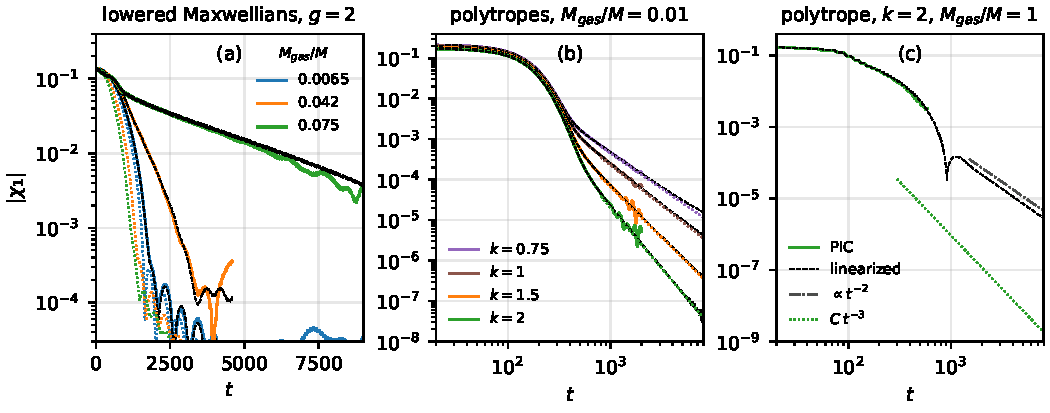
\includegraphics[width=\textwidth]{figuras/resultados_amortiguado.pdf}}
\caption{Response of the gas to the perturbation~(\ref{Eq:InitialData}) for steady states without oscillating mode. (a) Lowered Maxwellians with $g = 2$ and $J_{max} = 0.138$ below the threshold mass. The solid lines are the results of the PIC simulations (with $\varepsilon = 1$, $0.065$ and $0.075$ in the order of increasing mass), the dashed lines the solutions of the linearized equations, and the dotted lines the solutions which are obtained when the self-gravity of the perturbation is omitted. (b) Polytropes with $M_{gas}/M = 0.01$. The solid lines are the results of the PIC simulations with $\varepsilon = 0.1$, which are shown for $t\leq 2000$, the dashed lines the solutions of the linearized equations, and the dotted lines the asymptotic expression~(\ref{Eq:TailChi}) for the mixing in a fixed potential. (c) Polytrope with $k = 2$ and $M_{gas}/M = 1$. Shown is the envelope of $|\chi_1|$ (largest value in a moving window of width $40$) for the PIC simulation with $\varepsilon = 0.1$, up to $t = 600$, and for the solution of the linearized equations with $N_J = 3200$. The dash-dotted line is proportional to $t^{-2}$, and the dotted line is the expression~(\ref{Eq:TailChi}).}
\label{Fig:Damped}
\end{figure}

Figure~\ref{Fig:Damped}(a) shows the function $|\chi_1(t)|$ for the lowered Maxwellians with $M_{gas}/M = 0.0065$, $0.042$ and $0.075$, for which $\lambda_{edge} = 0.100$, $0.555$ and $0.874$, respectively. In each case we show the result of the PIC simulation, the solution of the linearized equations~(\ref{Eq:LinVlasov},\ref{Eq:LinPoisson}), and the solution of Eq.~(\ref{Eq:LinVlasov}) without its third term. The latter describes the mixing of the perturbation in the fixed potential $\Phi_{eq}$ of the steady state, when its own gravitational field is neglected, and it is given by Eq.~(\ref{Eq:hnFree}) with the frequencies $\Omega(J)$ which belong to $\Phi_{eq}$. In this case $|\chi_1|$ decays faster than exponentially and falls below one percent of its initial value at $t = 1510$, $1280$ and $1130$ for the three masses. The self-gravity of the perturbation delays the decay: when it is taken into account, the same level is reached at $t = 1650$, $2650$ and $11300$, respectively. Hence, for the smallest mass the response is close to the one of the mixing in a fixed potential, whereas for $M_{gas}/M = 0.075$ the decay is ten times slower.

For $M_{gas}/M = 0.075$ the decay is exponential over more than two orders of magnitude, and the response is a damped oscillation of the form discussed at the end of section~\ref{SubSec:Edge}. Applying the method of section~\ref{SubSec:Fits} to the interval $2000\leq t\leq 4000$ we obtain $\omega = 0.07021\pm 6\times 10^{-5}$ and $\gamma = (3.4\pm 0.2)\times 10^{-4}$ from the solution of the linearized equations, and $\omega = 0.07028\pm 4\times 10^{-6}$ and $\gamma = (3.48\pm 0.06)\times 10^{-4}$ from the PIC simulation; in the intervals $1000\leq t\leq 2500$ and $4000\leq t\leq 7900$ the damping rate of the linearized solution is $(3.5\pm 0.6)\times 10^{-4}$ and $(3.7\pm 0.4)\times 10^{-4}$, respectively. The frequency lies inside the band, at $3$ percent of its width above the lower edge. For $t\gtrsim 1.4\times 10^4$, when the linearized solution has decreased by a factor of $300$, its decay becomes slower, which marks the transition to the algebraic tail. For $M_{gas}/M = 0.058$, where $\lambda_{edge} = 0.720$, the solution of the linearized equations yields $\omega = 0.0686$ and $\gamma = (1.1\pm 0.1)\times 10^{-3}$ in the interval $1300\leq t\leq 3900$, and the frequency lies $7$ percent of the width of the band above its lower edge. Therefore, as the threshold is approached from below, the frequency of the damped oscillation approaches the edge of the band and its damping rate tends to zero; above the threshold it becomes the oscillating mode which is analyzed in the next subsection. For $M_{gas}/M = 0.042$ and $0.0065$, in contrast, there is no interval in which the response is described by a single exponential function: for $M_{gas}/M = 0.042$ the rates which are obtained from the linearized solution in the consecutive intervals $460\leq t\leq 1380$ and $1380\leq t\leq 2760$ are $1.3\times 10^{-3}$ and $2.6\times 10^{-3}$.

In the three cases the PIC simulations reproduce the solutions of the linearized equations as long as the response exceeds the fluctuations of the reference simulation. In terms of the quantity~(\ref{Eq:kappa}), the ratio of the amplitudes lies between $1.000$ and $1.012$ for $M_{gas}/M = 0.0065$ and $555\leq t_0\leq 1665$, an interval at whose end $|\chi_1|$ has decreased to $8\times 10^{-3}$ of its initial value, between $0.998$ and $1.000$ for $M_{gas}/M = 0.042$ and $460\leq t_0\leq 1380$, and between $0.992$ and $0.997$ for $M_{gas}/M = 0.075$ and $1000\leq t_0\leq 2500$. In the last case $|\kappa|$ decreases to $0.96$ at $t_0 = 4000$ and to $0.93$ at $t_0 = 5000$. These values change by less than one percent when the number of particles is multiplied by four or the time step is halved; the difference is an effect of the finite amplitude of the perturbation, see section~\ref{SubSec:FixedLTrapping}.

Next, we consider the polytropes with $M_{gas}/M = 0.01$, which is the regime to which the results of Ref.~\cite{mHgRmScS25} refer. In this case the gain is small, except when $k\leq 1$ and the frequency is extremely close to the edge of the band: for $\delta\geq 10^{-3}$ it does not exceed $0.06$. Consequently, the response is dominated by mixing, and its behavior for large times is determined by the edge of the support of the DF. For the mixing in the fixed potential $\Phi_{eq}$, Eq.~(\ref{Eq:Tail}) applies with $\hat{F}_1 = \mathcal{F}_{0,eq}\, s/2$, which according to Eq.~(\ref{Eq:PolytropeEdge}) corresponds to $g(J_{max}) = \alpha\,\Omega_{min}^k B(J_{max})/2$ in Eq.~(\ref{Eq:EdgeBehavior}), and one obtains
\begin{equation}
|\chi_1(t)|\simeq \frac{C}{t^{k+1}},\qquad
C := \frac{\Gamma(k+1)\,\alpha\,\Omega_{min}^k B(J_{max})}{2\,|\Omega'(J_{max})|^{k+1}\int_0^{J_{max}} \mathcal{F}_{0,eq}(J) B(J)\, dJ},\qquad t\to \infty.
\label{Eq:TailChi}
\end{equation}
We have verified this expression by solving Eq.~(\ref{Eq:LinVlasov}) without its third term on a lattice with $N_J = 3200$ rows. The envelope of the resulting function $|\chi_1(t)|$ exceeds the right-hand side of Eq.~(\ref{Eq:TailChi}) by $8$, $9$, $12$ and $14$ percent at $t = 2000$ and by $4$, $4$, $5$ and $6$ percent at $t = 4000$ for $k = 0.75$, $1$, $1.5$ and $2$, respectively, and the results for $N_J = 1600$ agree with these values to within $0.3$ percent. The difference decreases in time approximately like $1/t$, as expected for the next term of the asymptotic expansion. (For $k = 2$ this only holds up to $t\approx 5000$; afterwards the solution approaches its numerical floor, which is of the order of $10^{-7}|\chi_1(0)|$.)

The self-gravity of the perturbation modifies this behavior. To see how, we expand $\delta\mathcal{F}_0$ and $\delta\Phi(t,r(Q,J))$ in Fourier series with respect to $Q$, with coefficients $\delta\hat{F}_n(t,J)$ and $\phi_n(t,J)$, respectively. Equation~(\ref{Eq:LinVlasov}) then yields $\partial_t\delta\hat{F}_n + in\Omega\,\delta\hat{F}_n = in\,\mathcal{F}_{0,eq}'\phi_n$, whose solution is
\begin{equation}
\delta\hat{F}_n(t,J) = e^{-in\Omega(J)t}\left[ \delta\hat{F}_n(0,J) + in\,\mathcal{F}_{0,eq}'(J)\,\hat{\Phi}_n(t,J) \right],\qquad
\hat{\Phi}_n(t,J) := \int\limits_0^t \phi_n(t',J) e^{in\Omega(J)t'} dt'.
\label{Eq:Duhamel}
\end{equation}
Hence, the perturbation evolves like in a fixed potential, but with an effective initial datum which accumulates the action of the perturbed potential on each orbit. The important point is that $\mathcal{F}_{0,eq}'$ vanishes like $(J_{max} - J)^{k-1}$ at the edge of the support, that is, one power more slowly than the initial perturbation. Suppose that $k > 1$ and that $\hat{\Phi}_1(t,J_{max})$ converges to a limit $\hat{\Phi}_\infty\neq 0$ for $t\to \infty$. Then, the argument which leads to Eq.~(\ref{Eq:Tail}), applied to both terms on the right-hand side of Eq.~(\ref{Eq:Duhamel}), gives
\begin{equation}
\chi_1(t)\simeq \chi_1^{mix}(t)\left[ 1 + 2|\Omega'(J_{max})|\,\hat{\Phi}_\infty\, t \right],
\label{Eq:TailSG}
\end{equation}
where $\chi_1^{mix}$ denotes the asymptotic expression for the mixing in the fixed potential, whose magnitude is given by Eq.~(\ref{Eq:TailChi}). Therefore, for times which are large compared to $t_\times := (2|\Omega'(J_{max})||\hat{\Phi}_\infty|)^{-1}$ the response decays like $t^{-k}$ instead of $t^{-(k+1)}$: the self-gravity of the perturbation reduces the exponent of the algebraic tail by one. In the derivation of Eq.~(\ref{Eq:TailSG}) we have treated $\hat{\Phi}_1(t,J)$ as a regular function of $J$ which is independent of $t$ at late times. This neglects the potential which is generated by the tail itself; hence, the amplitude of the second term is only correct to leading order in $M_{gas}/M$. For a discussion of algebraic tails of the linearized response in a one-dimensional model we refer the reader to Ref.~\cite{jBaOyY11}.

The solutions of the full linearized equations for $M_{gas}/M = 0.01$ are shown in Fig.~\ref{Fig:Damped}(b). For $k = 1.5$ and $k = 2$ the function $\hat{\Phi}_1(t,J_{max})$, which we compute from the potential along the outermost rows of the lattice, changes by less than half a percent for $t\geq 2000$; its magnitude is $2.5\times 10^{-4}$ and $1.45\times 10^{-4}$, respectively, which corresponds to $t_\times = 3.5\times 10^4$ and $6.0\times 10^4$, and its phase differs from $\pi/2$ by less than $0.01$, such that the two terms in Eq.~(\ref{Eq:TailSG}) add in quadrature. Consequently, at $t = 8000$ the second term only increases the magnitude of the response by three and one percent, respectively, and in the time span considered here the tail follows the law of the mixing in a fixed potential: the exponents which are obtained from a fit of the envelope in the interval $2000\leq t\leq 4000$ are $-2.58$ and $-3.10$, with and without self-gravity. (At these times the exponents still differ from $-(k+1)$ because of the correction of the order $1/t$ mentioned above.) The ratio between the envelopes with and without self-gravity is almost constant: for $1000\leq t\leq 4000$ it lies between $1.04$ and $1.06$ for $k = 1.5$ and between $1.03$ and $1.04$ for $k = 2$.

For $k\leq 1$ the situation is different, since $\hat{\Phi}_1(t,J_{max})$ does not converge. For $k = 0.75$ its magnitude grows from $7.9\times 10^{-4}$ at $t = 2000$ to $8.2\times 10^{-4}$ at $t = 8000$, and the second term in Eq.~(\ref{Eq:TailSG}), evaluated with $\hat{\Phi}_1(t,J_{max})$ in place of $\hat{\Phi}_\infty$, has the magnitude $0.18$, $0.37$ and $0.75$ at $t = 2000$, $4000$ and $8000$. This term accounts for the difference with respect to the mixing in a fixed potential: the ratio between the envelopes with and without self-gravity grows from $1.06$ at $t = 2000$ to $1.13$ at $t = 4000$ and $1.35$ at $t = 8000$, and the quotient between the envelope and the right-hand side of Eq.~(\ref{Eq:TailChi}) from $1.13$ to $1.38$, whereas the quotient between the envelope and the magnitude of the right-hand side of Eq.~(\ref{Eq:TailSG}) stays between $1.11$ and $1.15$ in the whole interval $2000\leq t\leq 8000$. For $k = 1$ the second term has the magnitude $0.12$, $0.24$ and $0.47$ at the same times, and the ratio between the envelopes grows from $1.06$ to $1.09$ and $1.19$. Accordingly, the exponents in $2000\leq t\leq 4000$ are $-1.72$ for $k = 0.75$ and $-2.02$ for $k = 1$, compared to $-1.80$ and $-2.06$ without self-gravity. This slow growth is the only trace of the oscillating mode which we find for these steady states: as shown in the previous subsection, the mode itself lies at $\delta_d = 2.0\times 10^{-8}$ and $\delta_d\approx 10^{-98}$ from the edge. Therefore, over the time span considered here the perturbation decays for all the values of $k$, approximately like $t^{-(k+1)}$, and the dichotomy between $k\leq 1$ and $k > 1$ cannot be observed.

The PIC simulations agree with the solutions of the linearized equations until the response has decreased by about three orders of magnitude. As mentioned in section~\ref{SubSec:ValResponse}, for $t\leq 2000$ the difference between both is smaller than $1.2\times 10^{-4}|\chi_1(0)|$, and for $300\leq t_0\leq 1000$ the ratio $|\kappa|$ of the amplitudes lies between $0.99$ and $1.01$ for the four values of $k$. At $t = 2000$, however, the envelope of $|\chi_1|$ itself has decreased to $6.8\times 10^{-4}|\chi_1(0)|$ for $k = 0.75$ and to $1.7\times 10^{-5}|\chi_1(0)|$ for $k = 2$. Hence, the PIC simulations confirm the decay and the onset of the tail, whereas the exponents given above rely on the linearized equations.

Finally, we consider the polytrope with $k = 2$ and $M_{gas}/M = 1$, for which $\lambda_{edge} = 0.820$. Its response is shown in Fig.~\ref{Fig:Damped}(c). It starts with a damped oscillation: a fit in the interval $100\leq t\leq 400$ gives $\omega = 0.1668\pm 0.0008$ and $\gamma = (6.4\pm 0.8)\times 10^{-3}$ for the solution of the linearized equations, and $\omega = 0.1671\pm 0.0005$ and $\gamma = (6.4\pm 0.9)\times 10^{-3}$ for the PIC simulation with $\varepsilon = 0.1$. The frequency lies $4$ percent of the width of the band above its lower edge. For $t > 1500$ the linearized solution follows an algebraic tail which oscillates with the frequency $\Omega_{min}$. The exponent which is obtained from a fit of its envelope is $-2.07$ in the interval $2000\leq t\leq 4000$ and $-2.04$ in $4000\leq t\leq 8000$ for $N_J = 3200$ ($-2.07$ and $-2.02$ for $N_J = 1600$), while the envelope decreases from $2.8\times 10^{-4}|\chi_1(0)|$ to $1.6\times 10^{-5}|\chi_1(0)|$. Hence, for this mass the tail has the exponent $-k = -2$ of Eq.~(\ref{Eq:TailSG}), and not the exponent $-3$ of the mixing in a fixed potential, whose amplitude~(\ref{Eq:TailChi}) it exceeds by a factor of $400$ at $t = 2000$ and of $1500$ at $t = 8000$. In this case $t_\times = 65$. As expected, for $M_{gas}/M = 1$ Eq.~(\ref{Eq:TailSG}) does not reproduce the amplitude of the tail, which is about $13$ times larger than the one which results from the computed value $|\hat{\Phi}_\infty| = 0.047$. The same change of the exponent is found for the polytrope with $k = 1.5$ and $M_{gas}/M = 0.6$, for which $\lambda_{edge} = 0.759$: in this case the exponent of the envelope of the linearized solution is $-1.54$ in the interval $2000\leq t\leq 4000$ and $-1.52$ in $4000\leq t\leq 8000$, compared to the exponent $-2.5$ of the mixing in a fixed potential. \EJ{The PIC simulation for this case has $N = 10^4$ and $\varepsilon = 0.1$. It is to be replaced by the simulations with $N = 1.024\times 10^5$ and $\varepsilon = 0.03$ and $0.1$ which have been run on the cluster and whose analysis is pending.}


\subsection{Oscillating modes above the threshold}
\label{SubSec:FixedLModes}

\begin{figure}[htp]
\centerline{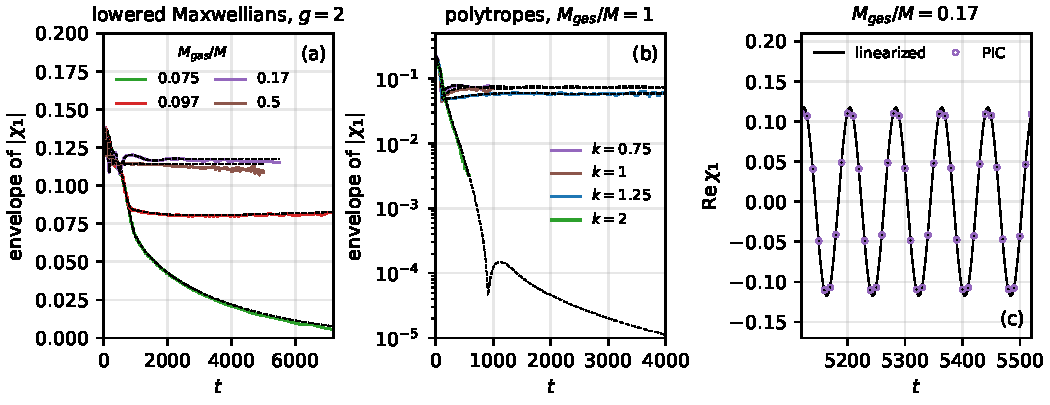
\includegraphics[width=\textwidth]{figuras/resultados_modos.pdf}}
\caption{Response of the gas for steady states above the threshold mass. (a) Envelope of $|\chi_1(t)|$ (largest value in a moving window of width $100$) for the lowered Maxwellians with $g = 2$ and $J_{max} = 0.138$, obtained from the PIC simulations with $\varepsilon = 0.075$, $0.01$, $0.1$ and $0.1$ in the order of increasing mass (solid lines) and from the linearized equations (dashed lines). The case $M_{gas}/M = 0.075$, which lies below the threshold, is included for comparison. (b) The same for the polytropes with $M_{gas}/M = 1$, with a window of width $50$. The PIC simulations have $\varepsilon = 0.1$ and are shown for $t\leq 1000$ ($t\leq 600$ for $k = 2$), except for $k = 1.25$, where $\varepsilon = 0.01$ and $N = 1.024\times 10^5$. (c) Real part of $\chi_1$ at the end of the simulation for the lowered Maxwellian with $M_{gas}/M = 0.17$.}
\label{Fig:Modes}
\end{figure}

When $\lambda_{edge} > 1$ the response does not decay. This is shown in Figs.~\ref{Fig:Modes}(a) and (b) for the lowered Maxwellians with $M_{gas}/M = 0.097$, $0.17$ and $0.5$ and for the polytropes with $k = 0.75$, $1$ and $1.25$ and $M_{gas}/M = 1$. After a transient, during which the part of the perturbation that does not belong to the mode undergoes mixing, the envelope of $|\chi_1|$ settles down to a constant value. For the lowered Maxwellians this value is $59$, $85$ and $83$ percent of $|\chi_1(0)|$ for the three masses, and for the polytropes it is $34$, $34$ and $30$ percent for the three values of $k$. The oscillation persists until the end of the linearized solutions, which comprise between $70$ and $100$ periods $2\pi/\omega_d$, and the PIC simulations follow them in amplitude as well as in phase, see Fig.~\ref{Fig:Modes}(c).

\begin{table}[htp]
\begin{center}
\begin{tabular}{ll|c|c|ccc}
\hline\hline
 & & $\Omega_{min}$ & $\delta_d$ & $\omega_d$ from Eq.~(\ref{Eq:ModeFrequency}) & linearized equations & PIC \\
\hline
lowered Maxwellian, $g = 2$ & $M_{gas}/M = 0.097$ & $0.072712$ & $0.0124$ & $0.072496$ & $0.072495$ & $0.072480$ \\
 & $M_{gas}/M = 0.17$ & $0.082745$ & $0.187$ & $0.078478$ & $0.078477$ & $0.078471$ \\
 & $M_{gas}/M = 0.5$ & $0.134193$ & $0.585$ & $0.104856$ & $0.104875$ & $0.104823$ \\
\hline
polytrope, $M_{gas}/M = 1$ & $k = 0.75$ & $0.151589$ & $0.0750$ & $0.141686$ & $0.141690$ & $0.14157$ \\
 & $k = 1$ & $0.153987$ & $0.0439$ & $0.147851$ & $0.147835$ & $0.14776$ \\
 & $k = 1.25$ & $0.156012$ & $0.0187$ & $0.153259$ & $0.153252$ & $0.153212$ \\
 & $k = 1.5$ & $0.157741$ & $0.00147$ & $0.157515$ & $0.157514$ & -- \\
\hline\hline
\end{tabular}
\end{center}
\caption{Frequency of the oscillating mode obtained from three different methods: the equation $\lambda(\omega_d) = 1$, a fit of the solution of the linearized equations, and a fit of the function $\chi_1(t)$ of the PIC simulations, both with the method of section~\ref{SubSec:Fits}. For the lowered Maxwellians the fits refer to the second half of the time span of the simulations, which extend to $t = 7200$, $5520$ and $5000$ and have the amplitudes $\varepsilon = 0.01$, $0.1$ and $0.1$, respectively. For the polytropes, the linearized solutions are fitted in the interval $1000\leq t\leq 4000$ ($8000\leq t\leq 14000$ for $k = 1.5$) and the PIC simulations in $300\leq t\leq 1000$ for $k = 0.75$ and $k = 1$ ($N = 10^4$, $\varepsilon = 0.1$) and in $500\leq t\leq 3900$ for $k = 1.25$ ($N = 1.024\times 10^5$, $\varepsilon = 0.01$).}
\label{Tab:Modes}
\end{table}

The frequencies of the oscillation are compared in Table~\ref{Tab:Modes}. Those which are obtained from the solutions of the linearized equations with the method of section~\ref{SubSec:Fits} agree with the roots of the equation $\lambda(\omega_d) = 1$ to within $2\times 10^{-5}$, that is, to within $2\times 10^{-4}$ in relative terms, and the damping rates which result from the same fits are smaller than $5\times 10^{-6}$ in magnitude, with either sign. The frequencies of the PIC simulations lie between $7\times 10^{-6}$ and $5\times 10^{-5}$ below $\omega_d$, except for the two simulations with $\varepsilon = 0.1$ and $N = 10^4$ of the polytropes, where the difference is about $10^{-4}$. The latter is consistent with the slight decrease of the frequency with the amplitude of the perturbation which was found in section~\ref{SubSec:ValResponse}. In all the cases the frequency of the oscillation lies below $\Omega_{min}$, and the distance between both is resolved by the three methods. Together with the results of the previous subsection this confirms the criterion of section~\ref{SubSec:Gain}: for the lowered Maxwellians with $g = 2$ and $J_{max} = 0.138$ the response is damped for $M_{gas}/M = 0.075$ and oscillates without damping for $M_{gas}/M = 0.097$, in accordance with the threshold $0.0906$ of Table~\ref{Tab:Threshold}, and for the polytropes with $M_{gas}/M = 1$ it oscillates for $k\leq 1.5$ and is damped for $k = 2$. \EJ{The PIC values for $k = 0.75$ and $k = 1$ are to be replaced by those of the simulations with $N = 1.024\times 10^5$ and $\varepsilon = 0.03$ which have been run on the cluster and whose analysis is pending.}

The polytrope with $k = 1.5$ and $M_{gas}/M = 1$ lies only slightly above the threshold mass $0.920$, and its mode is located at $\delta_d = 1.5\times 10^{-3}$. As discussed in section~\ref{SubSec:Edge}, in this situation a time of the order of $(\Omega_{min} - \omega_d)^{-1} = 4400$ is needed for the mode to separate from the contribution of the orbits near the edge. In fact, the envelope of the linearized solution decreases until $t\approx 4000$, from $0.031$ at $t = 500$ to $0.022$, and it has not settled down within the time span of the solutions considered so far. We have extended this solution to $t = 1.4\times 10^4$. For $4000\leq t\leq 14000$ the envelope varies slowly between $0.022$ and $0.025$, which corresponds to $12$ to $13$ percent of $|\chi_1(0)|$. The frequencies which are obtained from fits in the intervals $4000\leq t\leq 8000$ and $8000\leq t\leq 14000$ are $0.157513$ and $0.157514$, in agreement with $\omega_d = 0.157515$, and the corresponding damping rates are $7\times 10^{-6}$ and $5\times 10^{-7}$ in magnitude. A PIC simulation of this mode in the linear regime would require a much smaller amplitude than those used here, as we show next.


\subsection{Finite amplitude: trapping of the orbits near the edge}
\label{SubSec:FixedLTrapping}

In section~\ref{SubSec:ValResponse} we found that for the polytrope with $k = 1.25$ and $M_{gas}/M = 1$ the amplitude of the response falls below the one predicted by the linearized equations by an amount which depends on $\varepsilon$ and which is not a numerical artifact. In this subsection we show that this effect is caused by the gas particles near the edge of the steady state, which are trapped by the oscillating mode when its amplitude exceeds a critical value.

Consider the motion of a gas particle under the influence of an oscillating mode with frequency $\omega_d$. In terms of the action-angle variables of the steady state, this motion is governed by the Hamiltonian $H = E(J) + \delta\Phi(t,r(Q,J))$, see section~\ref{SubSec:Linearization}, and the expansion of section~\ref{SubSec:Gain} gives
\begin{equation}
\delta\Phi(t,r(Q,J)) = \varepsilon\sum\limits_{n\in\Integer} \phi_n(J) e^{i(nQ - \omega_d t)} + c.c.,
\label{Eq:ModePotential}
\end{equation}
where $\phi(r)$ refers to the mode which is excited by the perturbation~(\ref{Eq:InitialData}) with $\varepsilon = 1$ in the linear regime. For an orbit whose frequency $\Omega(J)$ is close to $\omega_d$, the term with $n = 1$ in Eq.~(\ref{Eq:ModePotential}) and its complex conjugate vary slowly along the unperturbed motion $Q = Q_0 + \Omega(J)t$, whereas all the other terms oscillate with frequencies which are at least of the order of $\omega_d$ and average out. Keeping only the former, writing $\phi_1(J) = |\phi_1(J)| e^{i\beta}$ and introducing the angle
\begin{equation}
\vartheta := Q - \omega_d t + \beta,
\label{Eq:thetaDef}
\end{equation}
which together with $J$ constitutes a set of canonical variables, one obtains the time-independent Hamiltonian
\begin{equation}
K(\vartheta,J) = E(J) - \omega_d J + 2\varepsilon |\phi_1(J)|\cos\vartheta.
\label{Eq:ResonantH}
\end{equation}
Let $J_r$ be the action variable of the resonant orbit, that is, $\Omega(J_r) = \omega_d$. Since $\omega_d < \Omega_{min}$ and $\Omega$ is a decreasing function, this orbit lies outside the support of the steady state, at the distance
\begin{equation}
d := J_r - J_{max}\approx \frac{\Omega_{min} - \omega_d}{|\Omega'(J_{max})|}
\label{Eq:dDef}
\end{equation}
from its edge. Expanding $E(J) - \omega_d J$ about $J = J_r$ to second order and neglecting the variation of $\phi_1$ and $\Omega'$ between $J_{max}$ and $J_r$, Eq.~(\ref{Eq:ResonantH}) yields, up to an additive constant,
\begin{equation}
K(\vartheta,J)\approx -\frac{1}{2}|\Omega'|(J - J_r)^2 + 2\varepsilon |\phi_1|\cos\vartheta,
\label{Eq:Pendulum}
\end{equation}
which is the Hamiltonian of a pendulum. Its level sets are separated into two classes by the separatrix
\begin{equation}
J = J_r\pm \Delta J_s\left| \cos\frac{\vartheta}{2} \right|,\qquad
\Delta J_s := \frac{2\omega_b}{|\Omega'|},\qquad
\omega_b := \sqrt{2\varepsilon |\phi_1| |\Omega'|}.
\label{Eq:Separatrix}
\end{equation}
A particle which lies inside the separatrix is trapped by the mode: its angle $\vartheta$ oscillates about zero, and its action variable oscillates about $J_r$ with an amplitude of up to $\Delta J_s$ and with a frequency which is equal to the bounce frequency $\omega_b$ close to the center $(\vartheta,J) = (0,J_r)$ and decreases towards the separatrix. Outside the separatrix $\vartheta$ varies monotonically. The same pendulum describes the particles which are trapped by a wave in a plasma, where it determines the nonlinear evolution of Landau damping~\cite{tO65}, and the orbits near a resonance in a galaxy~\cite{BinneyTremaine-Book}.

Initially, all the gas particles have $J\leq J_{max} < J_r$. Therefore, the effect of the mode on them depends on the ratio
\begin{equation}
s := \frac{\Delta J_s}{d} = \frac{2\omega_b}{\Omega_{min} - \omega_d}
\label{Eq:sDef}
\end{equation}
between the half-width of the separatrix and the distance of the resonance from the edge. If $s < 1$, the separatrix does not reach the support of the steady state, and none of the gas particles is trapped. Their action variables oscillate, and it follows from Eq.~(\ref{Eq:Pendulum}) that the largest value which is attained by a particle with $J = J_{max}$ at $t = 0$ is $J_+ = J_{max} + d\,( 1 - \sqrt{1 - s^2} )$. If $s > 1$, the particles close to the edge whose angle $\vartheta$ lies in a suitable interval about zero are trapped, and those which start next to the separatrix are carried to its top, such that $J_+ = J_r + \Delta J_s = J_{max} + d\,(1 + s)$. Since $\omega_b$ is proportional to $\sqrt{\varepsilon}$, the condition $s > 1$ is equivalent to
\begin{equation}
\varepsilon > \varepsilon_c := \frac{(\Omega_{min} - \omega_d)^2}{8 |\phi_1| |\Omega'|}.
\label{Eq:epsc}
\end{equation}
Hence, the closer the frequency of the mode lies to the edge of the band, the smaller is the amplitude which is required for trapping to occur.

In order to evaluate these expressions we determine $\phi_1$ from the solution of the linearized equations. To this purpose we compute the first harmonic $(1/N_Q)\sum_b \delta\Phi(t,r_{ab}) e^{-iQ_b}$ of the perturbation of the potential along the outermost row $a = N_J$ of the lattice. Since the radius is an even function of $Q$, this quantity is real, and according to Eq.~(\ref{Eq:ModePotential}) it is equal to $2\,\re[\phi_1(J) e^{-i\omega_d t}]$ once the transient has decayed. We obtain $\phi_1$ from a least-squares fit of this function in an interval which comprises between $1000$ and $2000$ time units after the transient. The results are listed in Table~\ref{Tab:Pendulum}. They change by less than two percent when the fit is repeated in the subsequent interval of at least the same length, except for $k = 1.5$, where the change is seven percent, and the root mean square of the residual of the fit lies between $0.2$ and $2$ percent of the one of the function ($5$ percent for $k = 1.5$).

\begin{table}[htp]
\begin{center}
\begin{tabular}{ll|cccc|cc}
\hline\hline
 & & $\Omega_{min} - \omega_d$ & $|\Omega'(J_{max})|$ & $|\phi_1|$ & $\omega_b/\sqrt{\varepsilon}$ & $\varepsilon_c$ & $J_r/J_{max}$ \\
\hline
lowered Maxwellian, $g = 2$ & $M_{gas}/M = 0.097$ & $2.17\times 10^{-4}$ & $0.0976$ & $1.60\times 10^{-5}$ & $1.77\times 10^{-3}$ & $0.0037$ & $1.016$ \\
 & $M_{gas}/M = 0.17$ & $4.27\times 10^{-3}$ & $0.1193$ & $4.16\times 10^{-5}$ & $3.15\times 10^{-3}$ & $0.46$ & $1.26$ \\
 & $M_{gas}/M = 0.5$ & $2.93\times 10^{-2}$ & $0.2306$ & $1.31\times 10^{-4}$ & $7.78\times 10^{-3}$ & $3.6$ & $1.92$ \\
\hline
polytrope, $M_{gas}/M = 1$ & $k = 0.75$ & $9.90\times 10^{-3}$ & $0.1422$ & $7.51\times 10^{-4}$ & $1.46\times 10^{-2}$ & $0.115$ & $1.100$ \\
 & $k = 1$ & $6.14\times 10^{-3}$ & $0.1475$ & $5.76\times 10^{-4}$ & $1.30\times 10^{-2}$ & $0.056$ & $1.060$ \\
 & $k = 1.25$ & $2.75\times 10^{-3}$ & $0.1520$ & $4.06\times 10^{-4}$ & $1.11\times 10^{-2}$ & $0.015$ & $1.026$ \\
 & $k = 1.5$ & $2.3\times 10^{-4}$ & $0.1557$ & $1.45\times 10^{-4}$ & $6.7\times 10^{-3}$ & $3\times 10^{-4}$ & $1.002$ \\
\hline\hline
\end{tabular}
\end{center}
\caption{Parameters of the pendulum~(\ref{Eq:Pendulum}) which describes the motion of the gas particles near the edge of the steady state in the field of the oscillating mode: distance of the frequency of the mode from the edge of the band, derivative of the frequency of the orbits and magnitude of the first harmonic of the potential of the mode at the edge (for $\varepsilon = 1$), bounce frequency, critical amplitude~(\ref{Eq:epsc}) and action variable of the resonant orbit.}
\label{Tab:Pendulum}
\end{table}

The critical amplitude varies over four orders of magnitude. For the lowered Maxwellian with $M_{gas}/M = 0.5$ it is larger than one, such that trapping does not occur for the perturbation~(\ref{Eq:InitialData}), whereas for the modes which lie close to the edge it is very small: $\varepsilon_c = 0.0037$ for the lowered Maxwellian with $M_{gas}/M = 0.097$, and $\varepsilon_c = 0.015$ and $3\times 10^{-4}$ for the polytropes with $k = 1.25$ and $k = 1.5$. In particular, of the three amplitudes $\varepsilon = 0.01$, $0.03$ and $0.1$ which were compared in section~\ref{SubSec:ValResponse} for $k = 1.25$, the first one lies below the critical amplitude ($s = 0.81$) and the other two above it ($s = 1.40$ and $2.55$).

\begin{figure}[htp]
\centerline{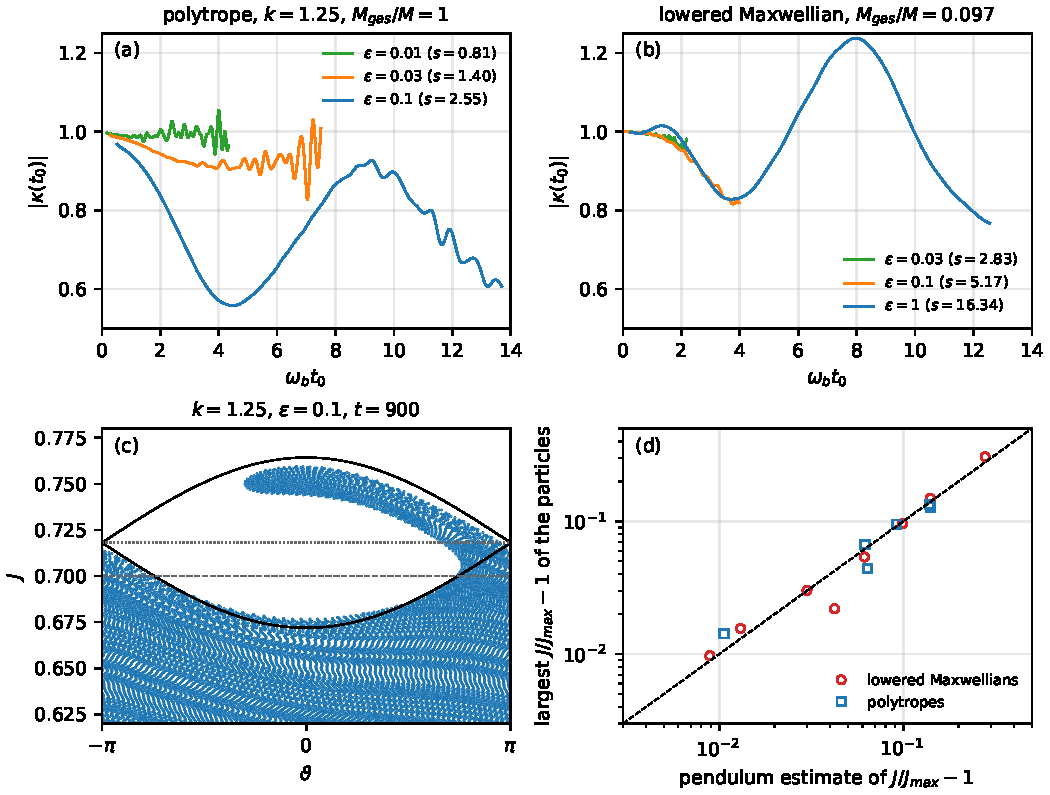
\includegraphics[width=0.85\textwidth]{figuras/resultados_atrapamiento.pdf}}
\caption{Effect of the amplitude of the perturbation on the oscillating mode. (a) Ratio $|\kappa(t_0)|$ between the amplitudes of the response obtained from the PIC code and from the linearized equations, see Eq.~(\ref{Eq:kappa}), as a function of time in units of the inverse bounce frequency, for the polytrope with $k = 1.25$ and $M_{gas}/M = 1$ and three amplitudes ($N = 1.024\times 10^5$). (b) The same for the lowered Maxwellian with $g = 2$ and $M_{gas}/M = 0.097$ ($N = 10^4$). (c) The computational particles near the edge of the steady state for the simulation with $\varepsilon = 0.1$ of panel (a) at $t = 900$, which corresponds to half a bounce period, in terms of the angle~(\ref{Eq:thetaDef}) and the action variable. The solid lines are the separatrix~(\ref{Eq:Separatrix}), the dashed line indicates $J_{max}$ and the dotted one $J_r$. (d) Largest value of the action variable attained by the computational particles in the simulations of Table~\ref{Tab:TrappingRuns}, compared to the value $J_+$ predicted by the pendulum~(\ref{Eq:Pendulum}).}
\label{Fig:Trapping}
\end{figure}

\begin{table}[htp]
\begin{center}
\begin{tabular}{ll|rc|cc|cc}
\hline\hline
 & & $\varepsilon$ & $s$ & $J_+$ (PIC) & $J_+$ (pendulum) & $\min|\kappa|$ & $\omega_b t_0$ \\
\hline
lowered Maxwellian, $g = 2$ & $M_{gas}/M = 0.097$ & $0.003$ & $0.89$ & $0.1393$ & $0.1392$ & $0.98$ & -- \\
 & & $0.01$ & $1.63$ & $0.1410$ & $0.1438$ & $0.98$ & $1.2^*$ \\
 & & $0.03$ & $2.83$ & $0.1454$ & $0.1465$ & $0.96$ & $2.1^*$ \\
 & & $0.1$ & $5.17$ & $0.1512$ & $0.1517$ & $0.82$ & $3.8^*$ \\
 & & $1$ & $16.3$ & $0.1802$ & $0.1765$ & $0.83$ & $3.7$ \\
 & $M_{gas}/M = 0.17$ & $0.1$ & $0.47$ & $0.1422$ & $0.1421$ & $0.99$ & -- \\
 & $M_{gas}/M = 0.5$ & $0.1$ & $0.17$ & $0.1402$ & $0.1398$ & $0.99$ & -- \\
 & & $1$ & $0.53$ & $0.1586$ & $0.1574$ & $1.00$ & -- \\
\hline
polytrope, $M_{gas}/M = 1$ & $k = 1.25$ & $0.01$ & $0.81$ & $0.7099$ & $0.7074$ & $0.98$ & -- \\
 & & $0.03$ & $1.40$ & $0.7467$ & $0.7434$ & $0.89$ & $5.4$ \\
 & & $0.1$ & $2.55$ & $0.7667$ & $0.7643$ & $0.56$ & $4.5$ \\
 & & $0.3$ & $4.42$ & $0.7897$ & $0.7981$ & $0.31$ & $4.1$ \\
 & $k = 1$ & $0.1$ & $1.34$ & $0.7941$ & $0.7975$ & $0.89$ & $3.6^*$ \\
 & $k = 0.75$ & $0.1$ & $0.93$ & $0.7308$ & $0.7446$ & $0.96$ & -- \\
\hline\hline
\end{tabular}
\end{center}
\caption{Simulations of steady states with an oscillating mode for different amplitudes of the perturbation: ratio~(\ref{Eq:sDef}), largest value of the action variable attained by the computational particles and its estimate $J_+$ from the pendulum~(\ref{Eq:Pendulum}), and smallest value of the ratio $|\kappa|$ between the amplitudes of the response of the PIC code and of the linearized equations. For $s > 1$ the latter refers to the interval $\omega_b t_0\leq 6$, and the last column gives the time at which it is attained; an asterisk indicates that this occurs at the end of the time span which is analyzed, such that $|\kappa|$ may decrease further. For $k = 1.25$ and $\varepsilon = 0.01$ the smallest value for $t_0\leq 2000$ is given. The simulations have $N = 10^4$ and are analyzed over their whole duration, except those of the polytropes with $k = 1.25$ and $\varepsilon\leq 0.1$, which have $N = 1.024\times 10^5$, and the remaining ones of the polytropes, which are only analyzed for $t\leq 1000$.}
\label{Tab:TrappingRuns}
\end{table}

These estimates are compared with the PIC simulations in Table~\ref{Tab:TrappingRuns} and Fig.~\ref{Fig:Trapping}. We first consider the motion of the particles. Figure~\ref{Fig:Trapping}(c) shows the computational particles with the largest values of the action variable for the polytrope with $k = 1.25$ and $\varepsilon = 0.1$ at $t = 900$, which corresponds to half a bounce period $\pi/\omega_b$. The particles which were located next to the edge with angles close to $\vartheta = 0$ have moved around the center of the island, and they reach $J = 0.76$, while the top of the separatrix lies at $J_r + \Delta J_s = 0.764$. The largest value of the action variable which is attained in the course of the simulation is $0.7099$, $0.7467$ and $0.7667$ for $\varepsilon = 0.01$, $0.03$ and $0.1$, respectively, compared to the estimates $J_+ = 0.7074$, $0.7434$ and $0.7643$; in the reference simulation it is $0.7033$. In particular, the excursion beyond $J_{max}$ grows by a factor of five between $\varepsilon = 0.01$ and $\varepsilon = 0.03$, which reflects the onset of the trapping at $\varepsilon_c = 0.015$. The same agreement is found for the remaining simulations, see Fig.~\ref{Fig:Trapping}(d): for those with $s > 1$ which extend over at least two units of $1/\omega_b$, the measured excursion $J_+ - J_{max}$ differs from the estimate by at most $12$ percent. The simulation with $\varepsilon = 0.01$ for the lowered Maxwellian with $M_{gas}/M = 0.097$ ends at $\omega_b t = 1.3$, before the trapped particles have completed half a bounce period, and in this case the excursion has only reached half of the estimate. For $s < 1$, where the excursions are small, the relative deviations are larger, up to $34$ percent. We stress that the estimate does not contain any adjustable parameter.

Next, we consider the amplitude of the response, which we compare with the one of the linearized solution by means of the quantity~(\ref{Eq:kappa}). In the simulations with $s < 1$, $|\kappa|$ stays between $0.98$ and $1.01$ for the lowered Maxwellians, and for the polytrope with $k = 1.25$ and $\varepsilon = 0.01$ it lies between $0.977$ and $1.005$ for $t_0\leq 2000$ (see section~\ref{SubSec:ValResponse}). For $s > 1$, in contrast, the amplitude falls below the linear one on the time scale $1/\omega_b$ and passes through a minimum at $\omega_b t_0\approx 4$, see Figs.~\ref{Fig:Trapping}(a) and (b). For the polytrope with $k = 1.25$ and $\varepsilon = 0.1$ the minimum is $0.56$ at $\omega_b t_0 = 4.5$; for $\varepsilon = 0.03$, where $s = 1.40$ is closer to the critical value, $|\kappa|$ decreases to $0.90$ at $\omega_b t_0 = 4.4$ and stays between $0.89$ and $0.95$ up to $\omega_b t_0 = 6.5$. For the lowered Maxwellian with $M_{gas}/M = 0.097$, the curves for $\varepsilon = 0.03$, $0.1$ and $1$, for which $s$ lies between $2.8$ and $16$, coincide with each other to within four percent when they are represented as functions of $\omega_b t_0$, as far as each simulation extends. In the simulation with $\varepsilon = 1$, which covers almost thirteen units of $1/\omega_b$, the minimum $|\kappa| = 0.83$ at $\omega_b t_0 = 3.7$ is followed by a maximum of $1.24$ at $\omega_b t_0 = 8.0$, after which $|\kappa|$ decreases again, to $0.77$ at the end of the simulation. Hence, the amplitude of the mode oscillates with a period which is about $1.4$ times the bounce period $2\pi/\omega_b$. Such oscillations are characteristic for a wave which interacts with trapped particles~\cite{tO65}. The results for $\varepsilon = 0.1$ and $M_{gas}/M = 0.097$ do not change when the number of particles is multiplied by four or the time step is halved: at $\omega_b t_0 = 3$ we obtain $|\kappa| = 0.872$, $0.873$ and $0.872$, respectively.

The reason for the loss of amplitude is the following. According to Eq.~(\ref{Eq:ModeEq}), in the linearized theory the DF of the mode is proportional to $\mathcal{F}_{0,eq}'(J)\,\phi_1(J)/[\Omega(J) - \omega_d]$, which is largest for the orbits near the edge, where $\Omega(J) - \omega_d$ is smallest. This expression presupposes that the particles follow the unperturbed orbits. For the trapped particles this is not the case: their contribution to the density of the mode ceases to grow in phase with the potential and oscillates with the bounce period instead. Although these particles carry a very small fraction of the mass of the gas (in the simulation with $k = 1.25$ and $\varepsilon = 0.1$, the particles which reach $J > J_{max} + 0.003$ amount to $1.5\times 10^{-4} M_{gas}$), their weight in the mode is large due to the small denominator. This explanation is consistent with the fact that, at comparable values of $s$, the loss is larger for the polytrope with $k = 1.25$ than for the lowered Maxwellian with $g = 2$ (compare the rows with $s = 2.55$ and $s = 5.17$ in Table~\ref{Tab:TrappingRuns}), since in the former case the derivative of the DF vanishes more slowly at the edge. However, we do not have a quantitative theory for the depth of the minimum.

Finite amplitude effects are also present below the threshold, where the resonant orbit lies inside the support of the steady state. For the lowered Maxwellian with $M_{gas}/M = 0.075$, whose response in the linear regime is damped with the rate $\gamma = 3.4\times 10^{-4}$ (see section~\ref{SubSec:FixedLDamped}), we have performed a simulation with $\varepsilon = 0.84$ up to $t = 17200$. In this case the decay of the envelope of $|\chi_1|$ stops at $t\approx 2700$, when it has decreased to $22$ percent of its initial value. Afterwards the envelope grows to $52$ percent at $t\approx 6500$, decreases to $18$ percent at $t\approx 11500$ and grows again; the same values are obtained with four times as many particles and with half the time step up to $t = 5000$. The period of this oscillation, about $8900$, is comparable to the bounce period $2\pi/\omega_b = 7700$ which results from Eq.~(\ref{Eq:Separatrix}) with the mean amplitude of the potential in the interval $4000\leq t\leq 17200$. This is the saturation of Landau damping by the trapping of the resonant particles which was predicted by O'Neil~\cite{tO65} for a plasma wave: the damping stops once the bounce frequency exceeds the damping rate.

We conclude that the linear regime of an oscillating mode is restricted to amplitudes $\varepsilon\ll \varepsilon_c$. For the modes which emerge at the threshold this is a severe restriction, since $\varepsilon_c$ vanishes quadratically with the distance $\Omega_{min} - \omega_d$ of the mode from the band. \EJ{The simulations of this subsection for $k = 0.75$ and $k = 1$ have $N = 10^4$ and $\varepsilon = 0.1$, and their analysis is restricted to $t\leq 1000$. They are to be replaced by the simulations with $N = 1.024\times 10^5$ and $\varepsilon = 0.03$ and $0.1$ which have been run on the cluster and whose analysis is pending; according to Table~\ref{Tab:Pendulum}, $\varepsilon = 0.03$ lies below the critical amplitude in both cases.}
